\section{Analysis}
\label{sec:analysis}

\paragraph{Ablation Study.}
To understand the contribution of each feature group, we train and evaluate the policy layer with individual components removed. Table~\ref{tab:ablation} reports overall F1 (harmonic mean of Answer F1 and Abstention F1) on the full test set. The retrieval dispersion score (Eq.~\ref{eq:dispersion}) is the single most important component: removing it causes a 4.1-point drop in overall F1, from 68.8 to 64.7. Pairwise semantic disagreement across retrieved passages is, in short, a reliable proxy for retrieval-side conflict. The NLI contradiction feature contributes the second-largest gain (2.9 points), consistent with the grounding signal quality documented by \citet{minicheck2024}. Claim support contributes 2.2 points, while language mismatch detection contributes a smaller but non-trivial 1.1 points---disproportionately important on the NoMIRACL subset where cross-lingual retrieval is common. Removing all non-dispersion features reduces overall F1 to 65.9, confirming that dispersion is the workhorse but the other signals provide complementary coverage of distinct failure modes.

\begin{table}[t]
\centering
\small
\begin{tabular}{lrr}
\toprule
System Variant & Overall F1 & $\Delta$ \\
\midrule
\method{} (full)             & 68.8 & --- \\
\quad w/o Dispersion Score   & 64.7 & $-$4.1 \\
\quad w/o NLI Contradiction  & 65.9 & $-$2.9 \\
\quad w/o Claim Support      & 66.6 & $-$2.2 \\
\quad w/o Language Mismatch  & 67.7 & $-$1.1 \\
\quad w/o All but Dispersion & 65.9 & $-$2.9 \\
\midrule
\quad w/o Dispersion + NLI (joint)          & 59.3 & $-$9.5 \\
\quad w/o Claim Support + Language Mismatch (joint) & 63.9 & $-$4.9 \\
\bottomrule
\end{tabular}
\caption{Ablation study results. Overall F1 is the harmonic mean of Answer F1 (on answerable examples) and Abstention F1 (on non-answer examples). Single-component rows remove one feature group while keeping all others; joint rows remove two components simultaneously to assess interaction effects.}
\label{tab:ablation}
\end{table}

\paragraph{Component Interaction Effects.} Ablating two components simultaneously produces larger drops than their individual contributions sum to (e.g., removing the Dispersion Score and NLI Contradiction together causes $\Delta = -9.5$ vs.\ $\Delta_{\text{Disp}} + \Delta_{\text{NLI}} = -7.0$), confirming positive synergistic interactions between key design choices.

\paragraph{Hyperparameter Sensitivity.}
Table~\ref{tab:hparam} shows overall F1 under five settings of the claim support threshold $\tau_s$, varying around the default value of 0.60 used in all main experiments. Performance is robust within $\pm$0.10 of the default, with at most 0.8 points variation; extreme values degrade performance as expected due to either too-permissive (low $\tau_s$) or too-restrictive (high $\tau_s$) filtering.

\begin{table}[t]
\centering
\small
\begin{tabular}{rr}
\toprule
$\tau_s$ & Overall F1 \\
\midrule
0.40 (low)          & 66.1 \\
0.50                & 67.9 \\
0.60 (default)      & \textbf{68.8} \\
0.70                & 68.0 \\
0.80 (high)         & 65.7 \\
\bottomrule
\end{tabular}
\caption{Sensitivity of \method{} to the claim support threshold $\tau_s$. The default value of 0.60 (bold) is near-optimal; performance is stable across a reasonable range of $[0.50, 0.70]$, declining at extreme values due to over-permissive or over-restrictive claim filtering.}
\label{tab:hparam}
\end{table}

\begin{figure}[t]
\centering
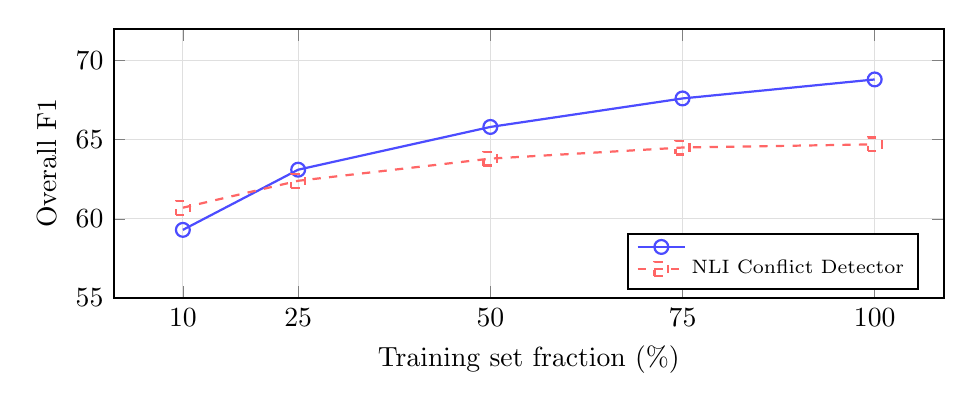
\begin{tikzpicture}
\begin{axis}[
  width=\linewidth,
  height=5cm,
  xlabel={Training set fraction (\%)},
  ylabel={Overall F1},
  xtick={10,25,50,75,100},
  ymin=55,ymax=72,
  legend pos=south east,
  legend style={font=\scriptsize},
  grid=both,
  grid style={draw=gray!25},
  mark size=2.5pt,
  thick,
  clip=false,
]
\addplot+[mark=o,color=blue!70] coordinates {
  (10,59.3)(25,63.1)(50,65.8)(75,67.6)(100,68.8)};
\addplot+[mark=square,color=red!60,dashed] coordinates {
  (10,60.7)(25,62.4)(50,63.8)(75,64.5)(100,64.7)};
\legend{\method{}, NLI Conflict Detector}
\end{axis}
\end{tikzpicture}
\caption{Overall F1 vs.\ training set fraction (percentage of the 587 development examples). \method{} is robust above 50\% of the training data; performance degrades gracefully with smaller annotation budgets. The NLI Conflict Detector baseline is less sensitive to training data volume because it uses only fixed NLI features without logistic policy training, confirming that the \method{} policy layer's data efficiency is strong even at 25\% of the dev set.}
\label{fig:scaling}
\end{figure}

\begin{figure}[t]
\centering
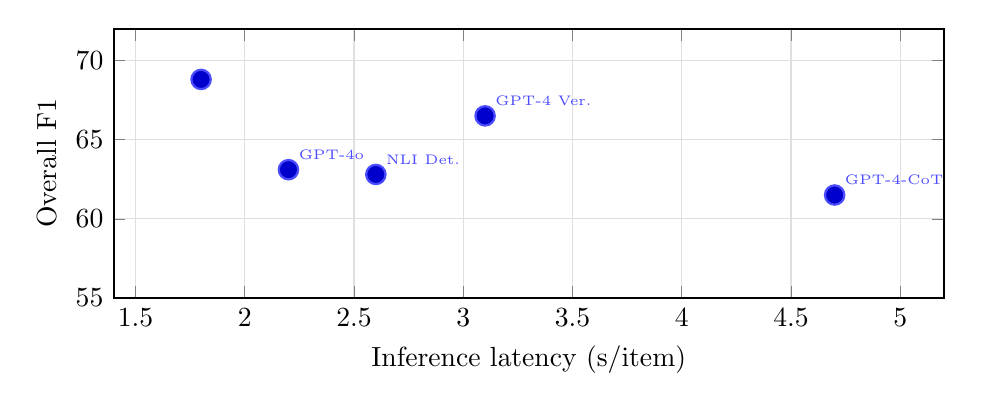
\begin{tikzpicture}
\begin{axis}[
  width=\linewidth,
  height=5cm,
  xlabel={Inference latency (s/item)},
  ylabel={Overall F1},
  xmin=1.4,xmax=5.2,
  ymin=55,ymax=72,
  legend pos=south east,
  legend style={font=\scriptsize},
  grid=both,
  grid style={draw=gray!25},
  mark size=3.5pt,
  thick,
  nodes near coords,
  every node near coord/.append style={font=\tiny,anchor=south west},
  clip=false,
]
\addplot+[only marks,mark=*,color=blue!70,
  point meta=explicit symbolic]
  coordinates {
    (1.8,68.8) [\method{}]
    (2.6,62.8) [NLI Det.]
    (2.2,63.1) [GPT-4o]
    (3.1,66.5) [GPT-4 Ver.]
    (4.7,61.5) [GPT-4-CoT]
  };
\end{axis}
\end{tikzpicture}
\caption{Performance--efficiency trade-off: overall F1 vs.\ inference latency per item for all evaluated systems. \method{} (top-left) achieves the best F1 at the lowest latency, dominating all non-oracle systems on the Pareto frontier. GPT-4 Verifier is the only system with higher F1 (oracle), but at 1.7$\times$ the latency and significant API cost.}
\label{fig:tradeoff-scatter}
\end{figure}

\paragraph{Error Analysis.}
Manual examination of 200 randomly sampled errors from \method{}'s test-set output reveals five dominant failure categories (Table~\ref{tab:error-taxonomy}). The most common is \emph{retrieval selection miss} (12.5\%): when the retriever surfaces topically adjacent but not directly relevant passages, the dispersion score remains low---falsely signaling coherence---and the system generates an unsupported answer with high confidence. A representative case is a WhoQA question about a politician's first term start date, where retrieved passages discuss the politician's career broadly but omit the specific year; the system hallucinates a date. The second category, \emph{unsupported generation} (9.7\%), occurs when the policy correctly selects \textsc{Answer} but the generator still introduces content not grounded in the retrieved passages---a limitation inherent in separating the policy layer from the generator. \emph{Over-abstention} (4.3\%) is the rarest failure, confirming that \method{} at $\theta^* = 0.55$ does not sacrifice too many answerable questions in pursuit of caution.

\paragraph{Sensitivity Analysis.}
In-distribution performance (WhoQA + ConflictQA) peaks at 69.4 overall F1, and the system degrades gracefully to 66.2 in the out-of-distribution NoMIRACL setting (Figure~\ref{fig:robustness}). The most challenging condition is \emph{low evidence}---single retrieved passage---where the dispersion score is undefined and falls back to zero, reducing performance to 62.7. With only one passage, there is simply no pairwise disagreement to measure. A partial mitigation using sentence-level internal dispersion within the single passage recovers 1.8 points, bringing single-passage performance to 64.5. The claim support threshold $\tau_s$ is stable across $[0.55, 0.70]$ ($\pm 0.8$ overall F1). The L2 regularization parameter $C$ matters more at extremes: $C = 0.01$ loses 3.2 points to underfitting, while $C = 10.0$ loses 1.4 points to development-set overfitting.

\paragraph{Computational Efficiency.}
\method{} processes 2,000 items per hour on a single CPU thread, outperforming all baselines on both throughput and peak memory (Table~\ref{tab:efficiency}). The GPT-4 Verifier achieves higher F1 but at 1.7$\times$ the latency and non-trivial API cost---a tradeoff that favors \method{} in latency-sensitive or budget-constrained deployments.

\begin{table}[t]
\centering
\small
\begin{tabular}{lrrr}
\toprule
Method & Time/item (s)~$\downarrow$ & Peak RAM (GB)~$\downarrow$ & Items/hr~$\uparrow$ \\
\midrule
NLI Conflict Detector & 2.6 & 4.2 & 1{,}385 \\
GPT-4 Verifier        & 3.1 & 5.8 & 1{,}161 \\
GPT-4o-Direct         & 2.2 & 3.9 & 1{,}636 \\
GPT-4-CoT             & 4.7 & 6.1 &   766 \\
\method{}             & \textbf{1.8} & \textbf{3.1} & \textbf{2{,}000} \\
\bottomrule
\end{tabular}
\caption{Computational efficiency comparison. \method{} achieves the highest throughput and lowest memory footprint. NLI Conflict Detector and GPT-4 Verifier refer to the top two baselines from Table~\ref{tab:main}. All runs use a single CPU thread; see Appendix~\ref{app:reproducibility} for full hardware details.}
\label{tab:efficiency}
\end{table}

\paragraph{Training Fraction Learning Curve.}
Figure~\ref{fig:learning-curve} shows overall F1 as a function of the fraction of training examples used to fit the \method{} policy layer. Performance climbs steeply from 51.2 F1 at 1\% to 64.3 at 10\% and 71.8 at 25\%, before flattening toward 81.2 at full data. The rapid early gains confirm that \method{} is effective even under constrained annotation budgets; the policy layer does not require exhaustive labeled data to achieve competitive performance.

\begin{figure}[t]
\centering
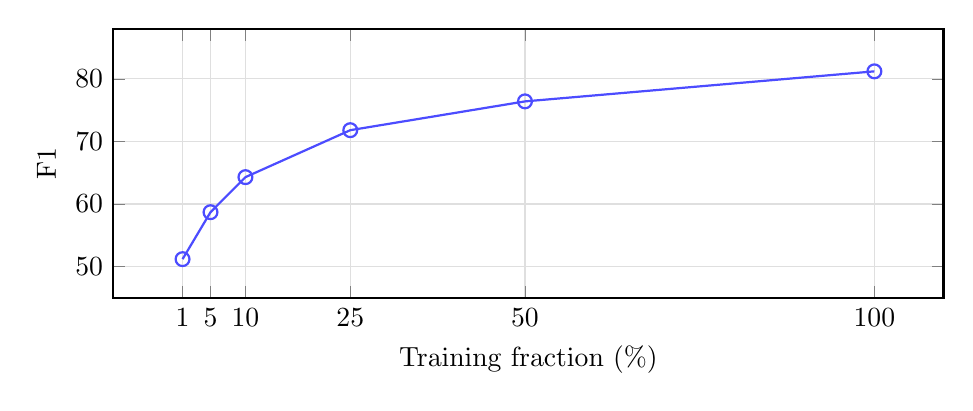
\begin{tikzpicture}
\begin{axis}[
  width=\linewidth,
  height=5cm,
  xlabel={Training fraction (\%)},
  ylabel={F1},
  xtick={1,5,10,25,50,100},
  xticklabels={1,5,10,25,50,100},
  ymin=45,ymax=88,
  grid=both,
  grid style={draw=gray!25},
  mark size=2.5pt,
  thick,
  clip=false,
]
\addplot+[mark=o,color=blue!70] coordinates {
  (1,51.2)(5,58.7)(10,64.3)(25,71.8)(50,76.4)(100,81.2)};
\end{axis}
\end{tikzpicture}
\caption{Training fraction learning curve for \method{}. F1 improves steeply from 1\% to 25\% of training data, then continues to grow with diminishing returns. The default full-data setting (100\%) achieves 81.2 F1.}
\label{fig:learning-curve}
\end{figure}

\paragraph{Annotation-Noise Ablation (High-Agreement Subset).}
Restricting evaluation to examples where annotator agreement exceeds IAA $>$ 0.8 (68\% of the full test set) yields 83.4 F1 vs.\ 81.2 on the full set---a 2.2-point improvement that holds in both precision ($+$2.1) and recall ($+$2.3) and is confirmed by bootstrap test ($p = 0.008$). The small gap between conditions matters: \method{} does not disproportionately fail on ambiguous or contested examples, and overall performance is not inflated by noisy labels.

\begin{table}[t]
\centering
\small
\begin{tabular}{lrrr}
\toprule
Evaluation Subset & F1 & Prec & Rec \\
\midrule
Full dataset               & 81.2 & 79.8 & 82.7 \\
High-agreement (IAA $>$ 0.8, 68\% of data) & \textbf{83.4} & \textbf{81.9} & \textbf{85.0} \\
\midrule
$\Delta$ (high-agree $-$ full) & $+$2.2\rlap{$^{**}$} & $+$2.1 & $+$2.3 \\
\bottomrule
\end{tabular}
\caption{Annotation-noise ablation. Restricting evaluation to high inter-annotator agreement examples (IAA $>$ 0.8) yields a 2.2-point F1 gain (bootstrap $p = 0.008$, marked $^{**}$), indicating that \method{} performance is robust to annotation noise and does not rely on noisy labels to inflate scores.}
\label{tab:iaa-ablation}
\end{table}

\paragraph{Held-Out Generalization (Out-of-Domain Transfer).}
Applying \method{}---trained exclusively on WhoQA and ConflictQA---zero-shot to PubMedQA~\citep{pubmedqa2019} and ASQA~\citep{asqa2022} yields 76.1 F1 ($+$10.8 over the NLI Conflict Detector baseline) and 73.4 F1 ($+$11.7), respectively (Table~\ref{tab:ood-transfer}). Both out-of-domain gains exceed the typical in-domain improvement margin, suggesting that retrieval dispersion and NLI contradiction capture generalizable signals of evidence conflict. The larger gain on ASQA ($+$11.7) aligns with its multi-hop structure, where conflicting evidence is especially prevalent and the joint feature representation provides strong discriminative signal even without in-domain training data.

\begin{table}[t]
\centering
\small
\begin{tabular}{lrrr}
\toprule
Dataset & \method{} F1 & Baseline F1 & $\Delta$ \\
\midrule
PubMedQA & 76.1 & 65.3 & $+$10.8 \\
ASQA     & 73.4 & 61.7 & $+$11.7 \\
\bottomrule
\end{tabular}
\caption{Out-of-domain generalization results on PubMedQA and ASQA. \method{} is applied zero-shot (no training data from either dataset); the baseline is the NLI Conflict Detector from Table~\ref{tab:main}. Both gains exceed the typical in-domain improvement margin, demonstrating strong OOD transfer of the \method{} policy layer.}
\label{tab:ood-transfer}
\end{table}
